%%%%%%%%%%%%%%%%%%%%%%%%%%%%%%%%%%%%%%%%%
% Wenneker Assignment
% LaTeX Template
% Version 2.0 (12/1/2019)
%
% This template originates from:
% http://www.LaTeXTemplates.com
%
% Authors:
% Vel (vel@LaTeXTemplates.com)
% Frits Wenneker
%
% License:
% CC BY-NC-SA 3.0 (http://creativecommons.org/licenses/by-nc-sa/3.0/)
%
%%%%%%%%%%%%%%%%%%%%%%%%%%%%%%%%%%%%%%%%%

%----------------------------------------------------------------------------------------
%	PACKAGES AND OTHER DOCUMENT CONFIGURATIONS
%----------------------------------------------------------------------------------------

\documentclass[11pt]{scrartcl} % Font size

%%%%%%%%%%%%%%%%%%%%%%%%%%%%%%%%%%%%%%%%%
% Wenneker Assignment
% Structure Specification File
% Version 2.0 (12/1/2019)
%
% This template originates from:
% http://www.LaTeXTemplates.com
%
% Authors:
% Vel (vel@LaTeXTemplates.com)
% Frits Wenneker
%
% License:
% CC BY-NC-SA 3.0 (http://creativecommons.org/licenses/by-nc-sa/3.0/)
%
%%%%%%%%%%%%%%%%%%%%%%%%%%%%%%%%%%%%%%%%%

%----------------------------------------------------------------------------------------
%	PACKAGES AND OTHER DOCUMENT CONFIGURATIONS
%----------------------------------------------------------------------------------------

\usepackage{amsmath, amsfonts, amsthm} % Math packages

\usepackage{listings} % Code listings, with syntax highlighting

\usepackage[english]{babel} % English language hyphenation

\usepackage[xetex]{graphicx}
%\usepackage{graphicx} % Required for inserting images
\graphicspath{{Figures/}{./}} % Specifies where to look for included images (trailing slash required)

\usepackage{booktabs} % Required for better horizontal rules in tables

\numberwithin{equation}{section} % Number equations within sections (i.e. 1.1, 1.2, 2.1, 2.2 instead of 1, 2, 3, 4)
\numberwithin{figure}{section} % Number figures within sections (i.e. 1.1, 1.2, 2.1, 2.2 instead of 1, 2, 3, 4)
\numberwithin{table}{section} % Number tables within sections (i.e. 1.1, 1.2, 2.1, 2.2 instead of 1, 2, 3, 4)

\setlength\parindent{0pt} % Removes all indentation from paragraphs

\usepackage{enumitem} % Required for list customisation
\setlist{noitemsep} % No spacing between list items

%----------------------------------------------------------------------------------------
%	DOCUMENT MARGINS
%----------------------------------------------------------------------------------------

\usepackage{geometry} % Required for adjusting page dimensions and margins

\geometry{
	paper=a4paper, % Paper size, change to letterpaper for US letter size
	top=2.5cm, % Top margin
	bottom=3cm, % Bottom margin
	left=3cm, % Left margin
	right=3cm, % Right margin
	headheight=0.75cm, % Header height
	footskip=1.5cm, % Space from the bottom margin to the baseline of the footer
	headsep=0.75cm, % Space from the top margin to the baseline of the header
	%showframe, % Uncomment to show how the type block is set on the page
}

%----------------------------------------------------------------------------------------
%	FONTS
%----------------------------------------------------------------------------------------

\usepackage[utf8]{inputenc} % Required for inputting international characters
\usepackage[T1]{fontenc} % Use 8-bit encoding

\usepackage{fourier} % Use the Adobe Utopia font for the document

%----------------------------------------------------------------------------------------
%	SECTION TITLES
%----------------------------------------------------------------------------------------

\usepackage{sectsty} % Allows customising section commands

\sectionfont{\vspace{6pt}\centering\normalfont\scshape} % \section{} styling
\subsectionfont{\normalfont\bfseries} % \subsection{} styling
\subsubsectionfont{\normalfont\itshape} % \subsubsection{} styling
\paragraphfont{\normalfont\scshape} % \paragraph{} styling

%----------------------------------------------------------------------------------------
%	HEADERS AND FOOTERS
%----------------------------------------------------------------------------------------

\usepackage{scrlayer-scrpage} % Required for customising headers and footers

\ohead*{} % Right header
\ihead*{} % Left header
\chead*{} % Centre header

\ofoot*{} % Right footer
\ifoot*{} % Left footer
\cfoot*{\pagemark} % Centre footer
 % Include the file specifying the document structure and custom commands
% LaTeX settings for MATLAB code listings
% based on Ted Pavlic's settings in http://links.tedpavlic.com/ascii/homework_new_tex.ascii
\usepackage{listings}
\usepackage[usenames,dvipsnames]{color}

% This is the color used for MATLAB comments below
\definecolor{MyDarkGreen}{rgb}{0.0,0.4,0.0}

% For faster processing, load Matlab syntax for listings
\lstloadlanguages{Matlab}%
\lstset{language=Matlab,                        % Use MATLAB
        frame=single,                           % Single frame around code
        basicstyle=\scriptsize\ttfamily,             % Use small true type font
        keywordstyle=[1]\color{Blue}\bfseries,        % MATLAB functions bold and blue
        keywordstyle=[2]\color{Purple},         % MATLAB function arguments purple
        keywordstyle=[3]\color{Blue}\underbar,  % User functions underlined and blue
        identifierstyle=,                       % Nothing special about identifiers
                                                % Comments small dark green courier
        commentstyle=\usefont{T1}{pcr}{m}{sl}\color{MyDarkGreen}\small,
        stringstyle=\color{Purple},             % Strings are purple
        showstringspaces=false,                 % Don't put marks in string spaces
        tabsize=3,                              % 5 spaces per tab
        %
        %%% Put standard MATLAB functions not included in the default
        %%% language here
        morekeywords={xlim,ylim,var,alpha,factorial,poissrnd,normpdf,normcdf,imresize,double,immse,fspecial,cell2mat,circshift,cell},
        %
        %%% Put MATLAB function parameters here
        morekeywords=[2]{on, off, interp},
        %
        %%% Put user defined functions here
        morekeywords=[3]{FindESS, homework_example},
        %
        morecomment=[l][\color{Blue}]{...},     % Line continuation (...) like blue comment
        numbers=left,                           % Line numbers on left
        firstnumber=1,                          % Line numbers start with line 1
        numberstyle=\tiny\color{Blue},          % Line numbers are blue
        stepnumber=1                            % Line numbers go in steps of 5
        }

% Includes a MATLAB script.
% The first parameter is the label, which also is the name of the script
%   without the .m.
% The second parameter is the optional caption.
\newcommand{\matlabscript}[2]
  {\begin{itemize}\item[]\lstinputlisting[caption=#2,label=#1]{#1.m}\end{itemize}}


\usepackage{fontspec}
\setmainfont{Tinos Nerd Font} %nice font for english and greek

\usepackage{hyperref} %for hyperlinks
\hypersetup{
    colorlinks=true,
    linkcolor=blue,
    filecolor=magenta,
    urlcolor=cyan,
}
%----------------------------------------------------------------------------------------
%	TITLE SECTION
%----------------------------------------------------------------------------------------

\title{
	\normalfont\normalsize
	\textsc{Technical University of Crete, ECE}\\ % Your university, school and/or department name(s)
	\vspace{25pt} % Whitespace
	\rule{\linewidth}{0.5pt}\\ % Thin top horizontal rule
	\vspace{20pt} % Whitespace
	{\Huge Digital Image Processing}\\ % The assignment title

	{\huge First Lab Report}\\ % The assignment title
	\vspace{12pt} % Whitespace
	\rule{\linewidth}{2pt}\\ % Thick bottom horizontal rule
	\vspace{12pt} % Whitespace
}

\author{\LARGE{Τσιαούσης Χρήστος}\\
		\texttt{2016030017}
		\and
		\LARGE{Πρωτοπαπαδάκης Γιώργος}\\
		\texttt{2016030134}}% Your name

\date{\normalsize\today} % Today's date (\today) or a custom date

\begin{document}

\maketitle % Print the title

%----------------------------------------------------------------------------------------
%	FIGURE EXAMPLE
%----------------------------------------------------------------------------------------

\section{Σκοπός Εργαστηρίου}

\begin{figure}[h] % [h] forces the figure to be output where it is defined in the code (it suppresses floating)
	\centering
	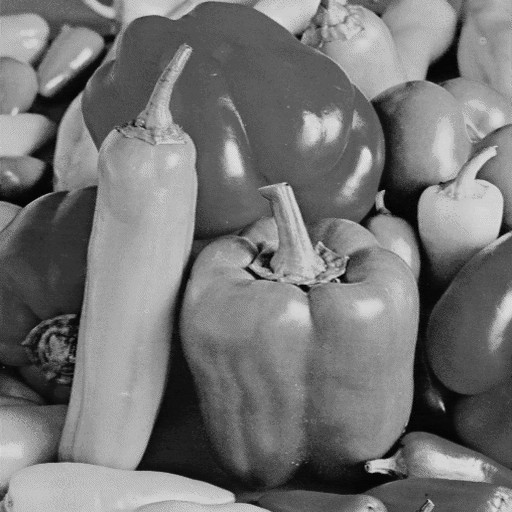
\includegraphics[width=0.5\columnwidth]{gray.jpg} % Example image
	\caption{Αρχική εικόνα.}
\end{figure}


Το εργαστήριο έχει να κάνει με την επιρροή του downsampling και upsampling στην πληροφορία της αρχικής εικόνας. Κάνοντας resize την εικόνα, ελέγχουμε "με το μάτι"
τις διαφορετικές επιδράσεις που έχει η εκάστοτε μέθοδος παρεμβολής \textit{(nearest-neighbor, bilinear, bicubic)} στις μικρότερες εικόνες. Έπειτα
επαναφέρουμε στο αρχικό μέγεθος και ελέγχουμε την τιμή του Μέσου Τετραγωνικού Σφάλματος (MSE).
%------------------------------------------------

\section{Xωρίς Αnti-Αliasing}

\subsection{Downsample}

Όπως φαίνεται στην παρακάτω φωτογραφία, μπορεί κανείς ακόμα και με το μάτι να καταλάβει ότι το bicubic interpolation κάνει καλύτερη δουλεία από
το bilinear, το οποίο επιβεβαιώνεται και από την θεωρία, καθώς το πρώτο έχει \textit{4x4 = 16 pixel Kernel} ενώ το δεύτερο έχει
\textit{2x2 = 4 pixel Kernel} με αποτέλεσμα να υπάρχουν πολύ λιγότερα artifacts με την χρήση του πρώτου. Ενώ με την μέθοδο nearest-neighbor,
έχουμε αρκετά περισσότερα artifacts καθώς η φύση του αλγορίθμου τίνει να γενικεύει και να καταλήγουμε με block από pixel τα οποία έχουν την ίδια τιμή.
Ίσως σε μια εικόνα αρκετά τετραγωνισμένη και μόνο με κατακόρυφες και οριζόντιες γραμμές, να βόλευε η πρώτη μέθοδος. Αν όμως υπάρχουν καμπύλες και
διαγώνιες, τότε σίγουρα χρειαζόμαστε μια μέθοδο που λαμβάνει υποψιν περισσότερα από ένα γειτονικά pixel όπως την πρώτη.

\begin{figure}[h] % [h] forces the figure to be output where it is defined in the code (it suppresses floating)
	\centering
	\includegraphics[width=\columnwidth]{1.jpg} % Example image
	\caption{Σύγκριση των διαφορετικών μεθόδων για σμίκρυνση εικόνας.}
\end{figure}

%----------------------------------------------------------------------------------------
%	TEXT EXAMPLE
%----------------------------------------------------------------------------------------

\subsection{Upsampling και Μέσο Τετραγωνικό Σφάλμα.}

Εδώ πρέπει να φανεί και περισσότερο η επίδραση του μεγέθους του Kernel για τις διαφορετικές μεθόδους.
Αρχικά, παρατηρούμε ότι όσο πιο πολύ μικραίνουμε μια εικόνα, τόσο πιο μεγάλο είναι το σφάλμα στην ανάκτησή της.
Επίσης, η πρόβλεψη που κάναμε για την απόδοση τις εκάστοτε μεθόδου είναι σωστή! Με την μόνη απόκληση να βρίσκεται
στην περίπτωση του x8 Upsampling μεταξύ των bilinear και bicubic, όπου η πρώτη μέθοδος εμφάνισε ελάχιστα μικρότερο σφάλμα.
Αυτό μπορεί να ωφείλεται στο ότι η bicubic μπορεί να παράγει τιμές για pixel εκτός των αρχικών διαστάσεων και αυτό για
μία τόσο μικρή εικόνα (64x64) είναι λογικό να αυξάνει το μέσο τετραγωνικό σφάλμα.

\begin{figure}[h] % [h] forces the figure to be output where it is defined in the code (it suppresses floating)
	\centering
	\includegraphics[width=\columnwidth]{2.jpg} % Example image
	\caption{Σύγκριση των MSE στις ανακτημένες εικόνες.}
\end{figure}


\newpage
%----------------------------------------------------------------------------------------
%	LIST EXAMPLES
%----------------------------------------------------------------------------------------

\section{Με Αnti-Αliasing}

\subsection{Downsample}

Η φιλοσοφία είναι ακριβώς η ίδια με το downsample που κάναμε στην πρώτη περίπτωση, μόνο που πλέον στα αποτελέσματα μπορούμε να παρατηρήσουμε
πολύ πιο λείες γραμμές, ειδικά για διαγψνίους. Η νέες εικόνες είναι πολύ πιο smooth αλλά και λόγω της μικρής τους ανάλυσης υπάρχει ένα ελαφρύ
θόλωμα. Η σύγκριση φαίνεται στο παρακάτω σχήμα:

\begin{figure}[h] % [h] forces the figure to be output where it is defined in the code (it suppresses floating)
	\centering
	\includegraphics[width=\columnwidth]{3.jpg} % Example image
	\caption{Σύγκριση των διαφορετικών μεθόδων για σμίκρυνση εικόνας, με Αnti-Αliasing.}
\end{figure}


%------------------------------------------------

\subsection{Upsampling και Μέσο Τετραγωνικό Σφάλμα.}

\begin{figure}[h] % [h] forces the figure to be output where it is defined in the code (it suppresses floating)
	\centering
	\includegraphics[width=\columnwidth]{4.jpg} % Example image
	\caption{Σύγκριση των MSE στις ανακτημένες εικόνες.}
\end{figure}

Βλέπουμε πως η μέθοδος Αnti-Αliasing κάνει πολύ πιο smooth τις γραμμές και τις καμπύλες και το αποτέλεσμα του upsampling είναι πολύ πιο ευχάριστο
στο μάτι. Ακόμα και στην μέθοδο nearest-neighbor έχει γίνει πολύ καλή δουλειά στην μείωση των ``rough edges´´ επάνω σε καμπύλες. Σε γενικές γραμμές
η πρώτη και τρίτη μέθοδος έχουν καθολικά μικρότερο σφάλμα. Ενδιαφέρον φαίνεται να έχει η περίπτωση του bilinear interpolation, καθώς το σφάλμα είναι
μεγαλύτερο για κάθε περίπτωση. Αυτό μπορεί να ωφείλεται στο ότι έχει μικρό Kernel και το Αnti-Αliasing φίλτρο μπορεί σε ορισμένα σημεία να έχει
δειγματολειπτήσει αρκετά αρεά ή αρκετά πυκνά, έτσι ώστε να πέρνουμε πάνω απο μία φορά τις τιμές ορισμένων pixel.

%----------------------------------------------------------------------------------------
%	TABLE EXAMPLE
%----------------------------------------------------------------------------------------

\section{Τελικά αποτελέσματα}

\begin{table}[h] % [h] forces the table to be output where it is defined in the code (it suppresses floating)
	\centering % Centre the table
	\begin{tabular}{l c c}
		\toprule
		\textit{μέθοδος (τιμή)} & \textbf{χωρίς Αnti-Αliasing} & \textbf{με Αnti-Αliasing} \\
		\midrule
		\midrule
		Neares-Neighbor (1/2) & 100 & 50\\
		Neares-Neighbor (1/4) & 198 & 132\\
		Neares-Neighbor (1/8) & 432 & 300\\
		\midrule
		BiLinear (1/2) & 38 & 48\\
		BiLinear (1/2) & 90 & 112\\
		BiLinear (1/2) & 230 & 265\\
		\midrule
		BiCubic (1/2) & 29 & 31\\
		BiCubic (1/4) & 86 & 77\\
		BiCubic (1/8) & 231 & 192\\
		\bottomrule
	\end{tabular}
	\caption{Τα τελικά σφάλματα.}
\end{table}


\section{Ο κώδικας που υλοποίησε τα παραπάνω}

\matlabscript {lab1}{Η υλοποίηση σε Matlab}

\section{References}


\begin{itemize}
  \item \href{https://en.wikipedia.org/wiki/Nearest-neighbor_interpolation}{Nearest-neighbor interpolation}
  \item \href{https://en.wikipedia.org/wiki/Bilinear_interpolation}{Bilinear interpolation}
  \item \href{https://en.wikipedia.org/wiki/Bicubic_interpolation}{Bicubic interpolation}
  \item \href{https://en.wikipedia.org/wiki/Anti-aliasing_filter}{Anti-aliasing filter}
\end{itemize}


\end{document}
